\documentclass{article}

\usepackage[utf8]{inputenc}
\usepackage[a4paper, total={6in, 8in}]{geometry}
\usepackage[shortlabels]{enumitem}
\usepackage{amsmath}
\usepackage{amssymb}
\usepackage{amsthm}
\usepackage{listings}
\usepackage{xcolor}
\usepackage{mathtools}
\usepackage{lmodern}
\DeclarePairedDelimiter\ceil{\lceil}{\rceil}
\DeclarePairedDelimiter\floor{\lfloor}{\rfloor}
\setlength{\parskip}{0.5em}

\usepackage{clrscode3e}

\title{Recursion: A Brief Introduction} 
\author{Competitive Programming UTEC}

\begin{document}

\maketitle

\section{Introduction}

\subsection{Definition}

\textbf{Recursion} occurs when a thing is defined in terms of itself or its type. This definition is a bit weird and doesn't tell us much, so lets consider the following problem. We want to define a rule set for balanced brackets. How would you define that rule set? Recursion allow us to have a very elegant and simple solution: We say that a sequence $L$ of brackets is balanced if $L = L_1(L_2)$, where $L_1$ and $L_2$ are balanced brackets, or $L$ is empty. By defining balanced brackets with smaller balanced brackets we can simplify how we describe what balanced brackets are. A nice definition of recursion therefore is:

\begin{center}
	\parbox{0.7\linewidth}{Recursion (rĭ-kûr’-zhn) \textit{noun.} If you still don't get it, see \textbf{recursion}.}
\end{center}

Recursion appears in many fields of knowledge such as mathematics, linguistics and computer science. This is due to the fact that it is a very powerful tool, that allows us to abstract concepts that might be hard to define and describe them in a very simple way. In computer science when we talk about recursion we usually refer to problems that can be solved by solving smaller instances of themselves. Now you might be asking: what makes a problem \textit{smaller} or \textit{bigger}? Intuitively, we say that a problem is bigger or harder if it takes more time to solve. For example, we can say that going up 5 stairs is harder than going up 3 stairs as we know that the more stairs there are, the longer it is going to take. A more formal definition would be that a problem is said to be smaller if it is fewer iterations away from the base case. This definition will probably make more sense as we further discuss the specifics and terminology of recursion.

\subsection{Conditions for Recursion}

There are three conditions that must be fulfilled for recursion to be possible:

\subsubsection{Recursive Call}

This is probably the easiest of all the conditions. It is obvious that in order to have a recursive algorithm at some point it must call the same algorithm but with different input, in other words, it must have a \textit{recursive call}. We can have more than one recursive call, or have the recursive calls inside conditionals, it is all fair game.

\subsubsection{Base Case}

Lets consider the following algorithm:

\begin{codebox}
\Procname{$\proc{factorial}(n)$}
	\li \Return  $n * \proc{factorial}(n - 1)$
\end{codebox}

It is simple to realize that there is one huge mistake in this algorithm: \textbf{it will never stop running!} This is why we need base cases, as they tell our algorithm when to stop. Formally a base case is a special behaviour inside the recursive algorithm that activates when it receives a specific parameter:

\begin{codebox}
\Procname{$\proc{factorial}(n)$}
\li \If $n = 0$
	\li \Then 
		\Return 1
	\End
\li \Return  $n * \proc{factorial}(n - 1)$
\end{codebox}

In this example the base case occurs when $n = 0$ and the function returns $1$. In general the base case can be anything that doesn't use recursion. In other words we must calculate the answer for the base case ``manually'' using an iterative approach. It is important to note that just as there can be more than one recursive call, there can also be more than one base case.

\subsubsection{Convergence}

This is probably the least intuitive of the three conditions, but it is still very simple to understand. Lets consider the following recursive algorithm:

\begin{codebox}
\Procname{$\proc{factorial}(n)$}
\li \If $n = 0$
	\li \Then 
		\Return 1
	\End
\li \Return $n * \proc{factorial}(n - 2)$
\end{codebox}

At first sight, it looks like this algorithm has no problems as there is a recursive call and a base case; however, there is a very important detail that has been overlooked. Lets say we call $\proc{factoria}(3)$, this would call $\proc{factorial}(1)$, which would call $\proc{factorial}(-1)$, which would call $\proc{factorial}(-3)$, and so on. Even though we had a base case, our algorithm \textbf{never reached it}, meaning it will be stuck in an infinite loop. This is not good. This is why \textit{convergence} is important, as it ensures that regardless of the parameters we use to call the algorithm, we should reach a base case after a finite number of steps. A corrected version of the algorithm above should consider two base cases, when $n$ reaches $0$ and when $n$ reaches $1$:

\begin{codebox}
\Procname{$\proc{factorial}(n)$}
\li \If $n \leq 1$
	\li \Then 
		\Return 1
	\End
\li \Return $n * \proc{factorial}(n - 2)$
\end{codebox}

\section{The Recursion Tree}

Lets consider the following algrithm for finding the $n$-th term of the Fibonacci sequence:

\begin{codebox}
\Procname{$\proc{fibonacci}(n)$}
\li \If $n \leq 1$
	\li \Then 
		\Return n
	\End
\li \Return $\proc{fibonacci}(n - 1) + \proc{fibonacci}(n - 2)$
\end{codebox}

What we are going to do now is build the \textit{recursion tree} for this algorithm. This is a graphical representation of how the recursive calls behave and interact, and are very usefull to anlayze the algorithms behaviour. In this case, for $n = 4$ the tree would look like this:

\begin{center}
	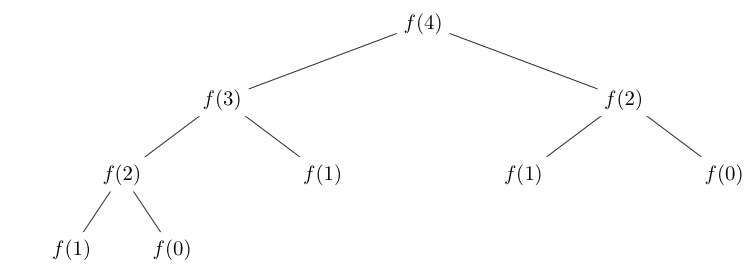
\includegraphics[width=0.8\linewidth]{images/fibtree}
\end{center}

Every node in this tree represents a call to the function $\proc{fibonacci}$, and the children of a node represents the recursive calls it make. The nodes that have no children are called leaf nodes, and in recursion trees they represent a base case. The first node is called the \textit{root} and it represents the first call to the algorithm.

Just by looking at this tree try to answer the following questions: Approximately how many nodes the tree will have for $n = 5$? What about for a general values of $n$?

\section{Complexity}

\subsection{Recurrence Relations}

Before we can jump into the algorithmic analysis we need to make a brief stop in the realm of discrete mathematics to understand recurrence relations. A \textit{difference equation} or \textit{recurrence relation} is an equation that tells us how different terms of a sequence relate. Lets consider the equation:

$$a_n = 2 a_{n - 1}, a_0 = 1$$

It is simple to see that this recurrence generates the sequence: $1, 2, 4, 8, 16, \dots 2^n \dots$ As you might have realized, this means that $a_n = 2^n$. This can be formally proved using \textit{mathematical induction}, but right now the intuition of why this is true is more than enough.

This process of turining a recurrence into a sequence defined only in terms of $n$ is usually called \textit{solving} the recurrence, we are esentially finding a recursion-free expression for the sequence. This is very usefull as for some large value of $n$ we don't need to solve for all the smaller values, we can just evaluate the expression. Another technique for solving recurrences is building a recursion tree and adding up to the solution. Some of this equations, like the example above, are very intuitive and simple to solve, while others are much more difficult and require advanced techniques.

\subsection{Time as a Recurrence} 

When dealing with iterative algorithms, calculating their time complexity was usually a very trivial task, we only needed to count the number of instructions that were going to be executed. This changes bit with recursion as it might be harder to tell how many times a given instruction will be executed, or how many times the recursive function will be called. For this reason, it is fitting that in order to analyze the time complexity of a recursive algorithm we use a recursive function. In general we can express the time complexity of a recursive algorithm as:

$$T(n) = \sum T(n_i) + T'(n)$$

Where $n_i$ is the parameter used to call the $i$-th recursive call ans $T'$ is the complexity of all non-recursive steps. Lets consider the previous code for finding factorials. We can see that in that case there is only one recursive call and a multiplication. This means that we can express the complexity of that code as:

$$T(n) = T(n - 1) + O(1)$$

This is a very straight forward recurrence that solves to $T(n) = O(n)$. Now lets do something a bit harder, lets try to determine the complexity of the algorithm for finding Fibonacci numbers. It is simple to realize that the complexity can be expressed as:

$$T(n) = T(n - 1) + T(n - 2) + O(1)$$

This recurrence is definitely trickier, so we must find another way of solving it. Lets remember that when we are using \textit{Big Oh} notation, we only want to find an estimate upper bound for the time complexity, therefore a good idea is to start by looking at the recursion tree and guessing. As in almost every step the number of nodes doubles, it is logical to guess that $T(n) = O(2^n)$. However, how can we prove this? A simple and straight forward way of doing it is by substituting our guess and checking:

$$T(n) = 2^{n - 1} + 2^{n - 2} + O(1)$$
$$T(n) \leq 2 * 2^{n - 1} + O(1)$$
$$T(n) \leq 2^n + O(1)$$
$$T(n) = O(2^n)$$

Even though this is not the most formal proof, it is enough to get an idea on how fast our solution will run. Later on, you will learn more advanced techniques for solving recurrences and estimating complexities.

Intuitively we can see that the more recursive calls we have, the bigger our time complexity will be. Therefore we must attempt to always minimize the number of recursive calls. We should also try to minimize the size of the smaller problems we target. However, this might be hard to achieve.

\subsection{Memory}

One important aspect to take into consideration when using recursion is that we are going to implicitly use memory of the stack. This happens because in every recursive call we need to store the current state of the algorithm in order to jump to the next function call. The auxiliary memory we will use in our algorithm will therefore be proportional to the height of our recursion tree, that is, the maximum distance between a leaf node and the root.

If we make too many recursive calls, this can lead to a stack overflow, in other words, we can run out of memory. This is one of the things that we must take into consideration when using recursion, as it can lead to our solution failing when dealing with bigger inputs.

\section{Strategy and Correctness}

Even though the problems that can be solved using recursion are very different, the solution for most of them follows a very similar pattern. First we find the solution for all the smaller problems we need, then we merge this solutions to find the general solution to the problem. Because of the versatility of recursion, lots of paradigms use it heavily.

Therefore the correctness of our algorithm depends on two things:
\begin{enumerate}
	\item \textbf{Base Case:} All of our base cases must give a correct result to our answer.
	\item \textbf{Merge:} The way in which we combine smaller solutions ensure that the general solution is also correct.
\end{enumerate}

One of the key advantages of this is that we can now give a lot more importance to the semantic meaning of our algorithms. This is to say that if we can describe what our algorithm does in words, whenever we use recursion in our solution we can assume that the result this yields is correct. For this reason recursion is a very abstraction heavy strategy that requires some practice in order to really get the most of this technique.


\end{document}
